\documentclass[letterpaper,11pt]{./templates/texMemo} % Set the paper size (letterpaper, a4paper, etc) and font size (10pt, 11pt or 12pt)

\usepackage{graphicx}
\graphicspath{ {../img/} }
\usepackage[parfill]{parskip} % Adds spacing between paragraphs
\setlength{\parindent}{0pt} % Indent paragraphs
\usepackage{float}

%----------------------------------------------------------------------------------------
%   MEMO INFORMATION
%----------------------------------------------------------------------------------------

\memoto{Calvin Engineering Advisory Council} % Recipient(s)

% Setup of the document
\memosubject{CEAC Design Report}
\memofrom{Team 14 - Daniel DeHoog, T.J. DeVries, Paul Griffioen, Ryan Siekman}

\memodate{April 11, 2016}

% Now the writing of the document can begin
\begin{document}

\maketitle 

\section{Project Description}
The goal of this project is to create a system that will allow people, both clients and administrators, to interact with gyms in a modern and smart way. This system will allow users to view what machines are currently open, and it will allow users to reserve machines for personal use. The system will also provide gym administrators with the ability to understand more clearly what machines get used, along with how often and when they are used.

\section{Marketability and Business Potential}
Currently, systems of a similar nature do not include all the features this product offers, and these systems cost significantly more money. This product will be flexible and modular, allowing gym administrators to both install the product on existing gym equipment and to only install pieces useful for their gym. Also, since the product is designed to be low cost and non-intrusive, it is a much more inexpensive upgrade than buying new equipment that has built-in reservation tracking. Because the product integrates into a central hub, all of the data is available for gym administrators to perform analytics on their data. With this data, gym administrators move their gym in the direction of a correct equipment distribution: buying more commonly used equipment and retiring less used equipment.

\section{System Overview}
Each machine in the gym is monitored by a sensor that communicates the status of the machine to a central hub. This information is relayed to a server and is viewed by the users via a website. The website also allows the users to create reservations, which are propagated back to the sensors and displayed on small LCD screens. Figure \ref{fig:general_overview} depicts a UML diagram of the system overview that is currently being implemented in the project.

\begin{figure}[H]
    \centering
    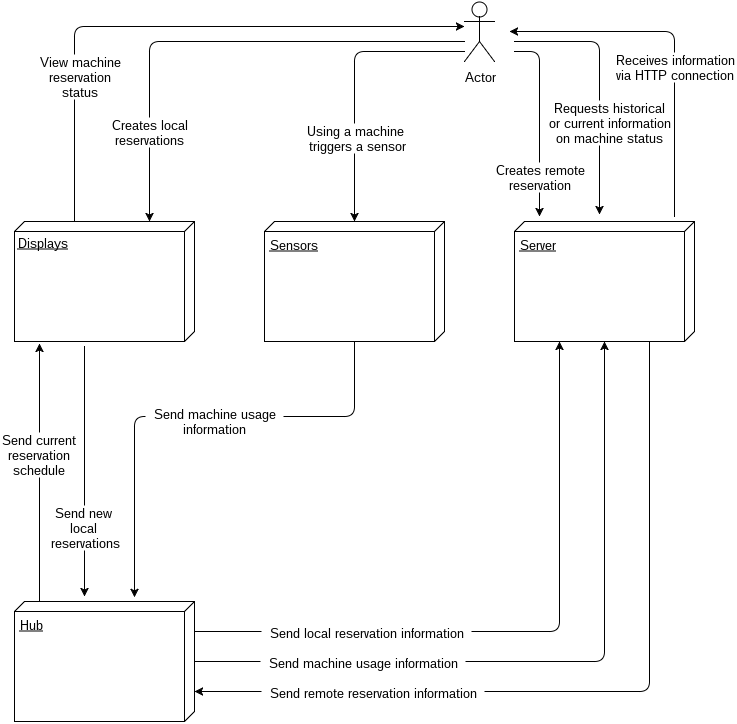
\includegraphics[width=\textwidth]{uml/general_overview.png}
    \caption{UML Diagram of the System Overview}
    \label{fig:general_overview}
\end{figure}

\section{Current Project Status}	

The team is currently working on developing the project in four major hardware areas. The work that has been completed and the work that still needs to be done is as follows:

\subsection{Sensors}
The team has successfully loaded custom code on the sensors (TI SensorTags) and is able to consistently read and process gyroscope, accelerometer, and device ID data over UART (universal asynchronous receiver/transmitter). In addition, the team has been able to implement a signal processing algorithm that analyzes the output and determines whether or not a machine is in use. The team is also able to turn off selected sensors on the SensorTag in addition to acquiring packets from the SensorTag using 6LoWPAN network communication. However, the SensorTags need to be configured to send packets containing gyroscope and accelerometer data, the SensorTag data output rate should be adjusted, and each SensorTag should output the current status of its battery.

\subsection{Displays}
The team has received all the necessary equipment to work with the displays, as well as the displays themselves, but has not yet started working with the on-machine display development. This is primarily because it is seen as a secondary function when compared to retrieving information from the sensors. There is, however, development for displaying information for all the machines. This will be discussed more in section 5.4.

\subsection{Hub}
The team has developed a system that is able to send rudimentary information about the current status of machines from the hub to the server. It is also able to retrieve information from the server and then get the packets ready to send onward to the sensors and displays. All of the logic is abstracted out so that whatever wrinkles are found during the development of the sensors and displays will be able to be on the outside of the hub development. This has allowed this development to continue parallel to the sensor and display development.

\subsection{Server}
The server's two main goals currently have functioning prototypes. There is a database implemented that can store users, machines, and their relationships, as well as a database model that abstracts out the implementation for other services to be able to use. There is a website that is currently being implemented that interfaces with the database model to get information specified by the requirements. This has working webpages, along with guidelines for what each page is required to do. There is a working login system, reservation system and it is now possible to have our sensors update the database in real-time based on the readings sent to the server.

\subsection{Summary}
The team has made progress that is on schedule with what is planned for the semester. The main goals left for the team are to start connecting each of the different areas, adding functionality on the user end, and implementing the on-machine displays.

\end{document}
